\chapter{IPv6}
\label{ch:IPv6}
\textbf{Internet Protocol version 6}, shortened with \textbf{IPv6}, is the most recent version of the Internet Protocol (IP). It was developed by the Internet Engineering Task Force (IETF) to deal with the long-anticipated problem of \textbf{IPv4 address exhaustion}, and is intended to fully replace IPv4.

%----------------------------------------------------------------------------------------

\section{History of IPv6}
The history of IPv6 began when it was clear that sooner or later no more IPv4 addresses would be available. In short, it is mostly made of people who realized that IPv4 was a bad idea, many contradictory predictions of when the IPv4 address pool would be depleted and ultimately other predictions about the full deployment of IPv6 (which turned out so wrong that at this rate we might never even see it happen in our lifetime, or something along these lines). A simplified timeline of the most important milestones in the life of this protocol follows.

%-------------------------------------------

\subsection{IPv4 address exhaustion}
\begin{figure}[h]
    \centering
    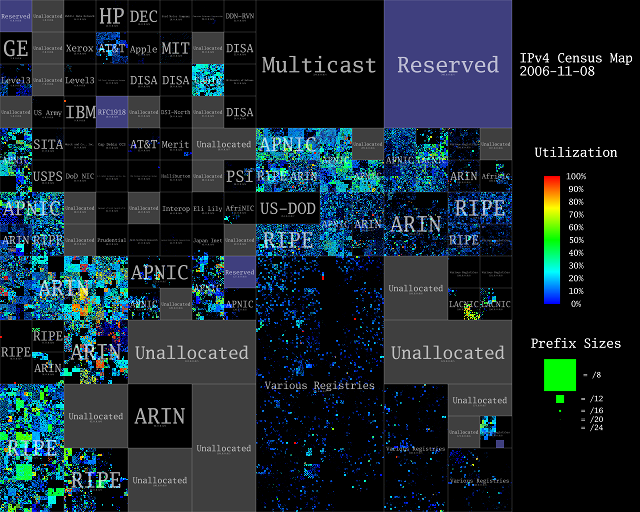
\includegraphics[scale=0.8]{img/ipv4_census_map.png}
    \decoRule
    \caption{IPv4 2006 census map, showing the distribution of IPv4 addresses.}
    \label{fig:ipv4_census_map}
\end{figure}

IPv4 address exhaustion is the depletion of the pool of unallocated IPv4 addresses. Because the original Internet architecture had fewer than 4,3 billion addresses available, depletion has been anticipated since the late '80s, when the Internet started experiencing dramatic growth.

Not all IPv4 are actually used, because many of them have been bought by people and companies who are not actually using them. However, their exhaustion was inevitable anyway because the Internet's growth has increased dramatically, not only for the high number of people who now have access to it but also because of the millions of devices online (like smartphones, IoT, etc.).

As of today (2020), IPv4 addresses are exhausted; however, they are still in wide use, so what does this mean?
Let us first understand who is consuming these addresses.

In order to use an IP address we have to \textit{own} it, and not a single one, but a block of them. So let us suppose that we are a business which, for legitimate reasons, want to have its own addresses. We go to a regional registry and ask for addresses; if there are available IPs, we pay a nominal cost (a small tax needed for the registry's operations) and get some for ourselves.

Until exhaustion, we could just go to a register and ask for a block of IP addresses; now, we have to wait in a line for weeks or months in order to obtain a new block. But wait - were not all addresses exhausted? Yes, but no: some companies that owned blocks have closed, or have released old blocks, so we can get a new one even if there are no new blocks available. Alternatively, we could also ask a company on the free market to sell their addresses to us\footnote{If UniFi would sell even just half of their IPv4 addresses, they would probably get enough money to renew a large number of their buildings: IPv4 addresses are extremely valuable.}.

On the contrary, if we want IPv6 addresses we just have to send an e-mail to the registry, and we will get as many as we want.

%-------------------------------------------

\subsection{IPv6 timeline}

\begin{figure}[H]
    \centering
    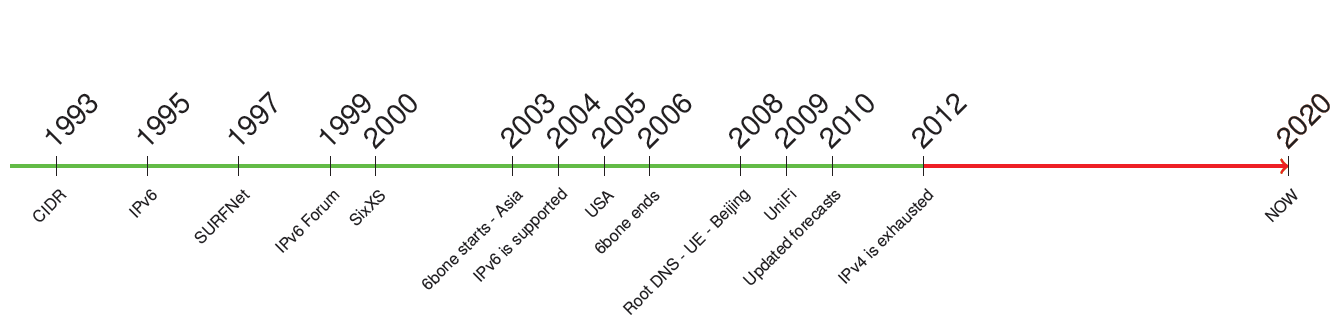
\includegraphics[scale=0.48]{img/ipv6timeline.png}
    \decoRule
    \caption{IPv6 timeline.}
    \label{fig:ipv6timeline}
\end{figure}

%----------------------

\subsubsection*{1993}
After realizing that that class-based routing was a bad idea, CIDR delays the exhaustion of IPv4 addresses by giving out smaller blocks. Before CIDR it was not possible to assign more than 254 addresses of class C (not even two consecutive block of this class), so people who required more IPs used to get a class B block, which was much larger. CIDR also helps reducing (dramatically) the routing table size.

%----------------------

\subsubsection*{1995}
IPv6 is officially released with RFC 1752. Note that as of today (2020), it is a 25-year old protocol, so not exactly a new one.

%----------------------

\subsubsection*{1997}
SURFNet, Netherlands’s academic network, goes fully IPv6.

%----------------------

\subsubsection*{1999}
IPv6Forum and regional task forces are created in order to force the adoption of IPv6; they fail miserably.

%----------------------

\subsubsection*{2000}
SixXS, one of the largest tunnel brokers, starts its operations, allowing users to connect their devices computer to the IPv6 network through it.

%----------------------

\subsubsection*{2003}
6bone, an IPv6 test bed\footnote{A \textbf{test bed} is the test execution environment configured for testing. Test beds consist of specific hardware, software, operating systems, network configurations, the product under test and other system software.}, is created to test worldwide IPv6. Japan, China and South Korea announce their willingness to become leaders in IPv6, mostly because they are heavily populated and connected to the Internet.

%----------------------

\subsubsection*{2004}
The majority of network nodes (routers) are supporting IPv6.

%----------------------

\subsubsection*{2005}
Things start to become more interesting: the USA government requires that all federal agencies migrate to IPv6 before 2008 (and they are successful). At the same time Sify, India's largest ISP, starts giving IPv6 connectivity to end users, for overpopulation reasons. Also, Tony Hain, of Cisco Systems, forecasts that between 2009 and 2016 we would say goodbye to IPv4 because of the address exhaustion.

%----------------------

\subsubsection*{2006}
6bone experiment ends successfully.

%----------------------

\subsubsection*{2008}
Root DNS can be reached also through IPv6. This is not very surprising, as DNS is nothing more than a database: no matter how we ask a query, it will answer. If we ask for a translation of an alphanumeric address, it will reply with the list of IPv4 and IPv6 addresses corresponding to that alpanumeric address. In the same year, the EU Commission sets a goal of 25\% population reached by IPv6 before 2010 (and miserably fails, because ISPs were not actually forced to do it). Meanwhile, China uses IPv6 to cover the Beijing Olympic Games; it is the biggest IPv6 use ever seen, and the transition from IPv4 is so seamless that nobody even noticed anything different.

%----------------------

\subsubsection*{2009}
The UniFi backbone goes IPv6, along with a DNS server and a webserver. % Unfortunately, unlike IPv4, the SIAF remains.\footnote{Tell me if I should remove this, but please be aware that I will be very sorry if I will have to.} % TODO Infila questa frecciatina da qualche parte pls

%----------------------

\subsubsection*{2010}
Geoff Huston forecasts update the IPv4 address exhaustion timeline to a date between September 2011 and May 2012. That also the end of the world is expected to happen during this same year, at least according to the Mayan calendar, is only a coincidence.

%----------------------

\subsubsection*{2012}
The IPv4 address pool is (finally) exhausted. The world does not end.

%----------------------

\subsubsection*{2020}
IPv6 is still being rolled out – without too many issues, but without enough security, either (it is dramatically troublesome). IPv4 addresses are still available, but there is a waiting line.

\begin{figure}[h]
    \centering
    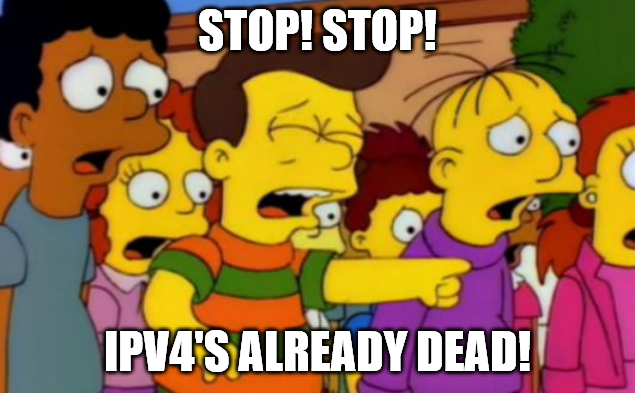
\includegraphics[scale=0.5]{img/ipv4_dead_meme.png}
    \decoRule
    \caption{IPv4 is dead, let it go.}
    \label{fig:ipv4_dead}
\end{figure}


%----------------------------------------------------------------------------------------

\section{IPv6 vs IPv4}
Since IPv6 is the new IP protocol version, its design goals are to fix the weak IPv4 points and enhance its strengths. It is very different and ultimately unrelated to IPv4, to the point that they can be compared to two parallel lines which never meet. For this reason, they can be used together as they will not mess up with each other (but neither will they be able to understand each other). The basic differences between them are:

\begin{enumerate}
    \item larger address space (128-bit addresses vs. IPv4 32-bit addresses\footnote{Someone could wonder why IPv4 addresses have such a short number of bits. The answer lies in the fact that no one expected the Internet to last for so long, nor to grow so fast and become as popular as it is nowadays (pretty much like nobody expects the Spanish Inquisition). It is, actually, the only case in the history of telecommunications of a network that keeps growing in time without becoming obsolete.});
    \item NATs are gone\footnote{Unless we are in extremely specific, almost non-existent contexts.};
    \item simplified packet header (dramatically faster);
    \item autoconfiguration.
\end{enumerate}

%-------------------------------------------

\subsection{Larger address space}
Suppose the green square in figure \ref{fig:ipv4_address_space} is the IPv4 address space; by comparison, the IPv6 address space would be represented by the white space around the green square, which in order to keep proportions we would have to extend outside the figure \textit{to the whole Solar System}. Another example: if we suppose an IP address to take the form of a standard grain of sand, measuring $1 mm$ x $1mm$ x $1mm$, in order to make the IPv4 address space we would need four and a half buckets of sand. For IPv6, we would need an amount of sand at least as the one necessary to cover the surfaces of six Earth planets (oceans included) with 1 $m$ of sand.

Such a humongous amount of addresses allow us to do something unthinkable in IPv4: waste them.

\begin{figure}[h]
    \centering
    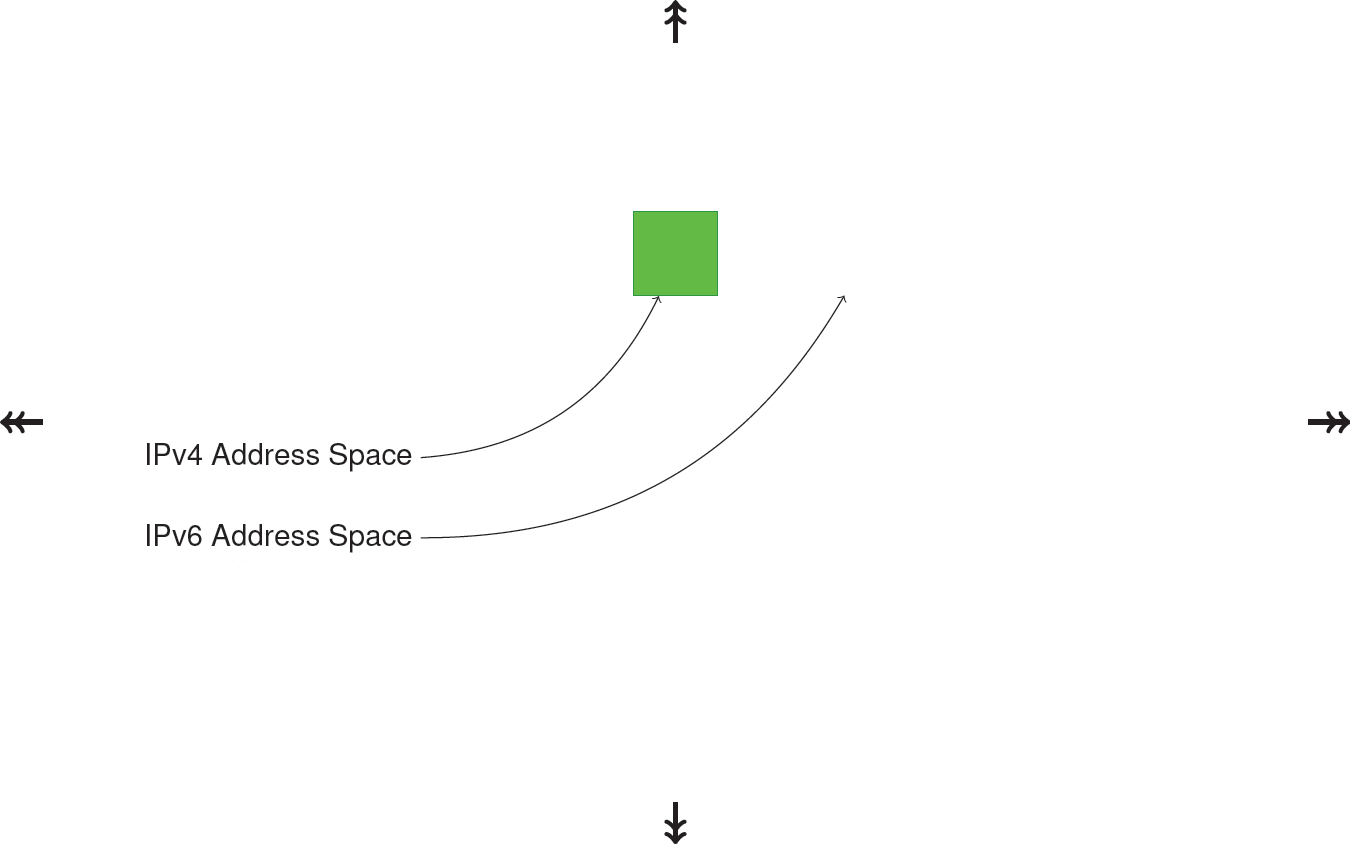
\includegraphics[scale=0.3]{img/ipv4_address_space.png}
    \decoRule
    \caption{IPv4 address space vs IPv6 address space comparison.}
    \label{fig:ipv4_address_space}
\end{figure}

%-------------------------------------------

\subsection{NATs}
In IPv4 every host connected to the Internet must have a unique address for routing. If it is not behind a NAT (Network Address Translation), then it will have a public, global address; otherwise, a host which is located in a subnet behind a NAT will have an IPv4 address which will not be unique in the global network, so it will not be able to use it for routing - in other words, the host will not be able to be reached from the outside directly.

As the name implies, NAT is an IP address mangling technique (a sort of rewriting of an IP address) used to allow multiple hosts to share the same (public) address. Basically, from the point of view of somebody outside the net, any amount of hosts behind a NAT will appear as a single IP address.

NAT allows a private IP address to reach Internet, but not the opposite - at least not in a predictable way: NATs are not deterministic, so it is not predictable if somebody from the Internet can reach a host behind one. It is also possible to bypass a NAT, even though through protocols that are either complex, difficult, dangerous or unstable.

\vspace{0.5em}

\emph{Example} The PS Remote Play application, which allows a user to play games on their PlayStation console remotely, uses techniques which allow it to bypass the NAT in order to reach the console directly - which in reality opens huge security flaws, much like creating a hole in the main door of a house.

\vspace{0.5em}

It is worth noting that we could be behind a NAT even if we have a public IP address, because sometimes ISPs use \textbf{Large Scale NATs} (LSN), very costly and unreliable machines.

To put it simply, NATs are something incredibly complex and ultimately useless, since they did not prevent the exhaustion of IPv4 addresses by limiting the number of devices directly connected to the Internet; they were also bad for security. It is thus a very positive thing that they do not exist anymore in IPv6.

%-------------------------------------------

\subsection{Simplified header}
\begin{figure}[h]
    \centering
    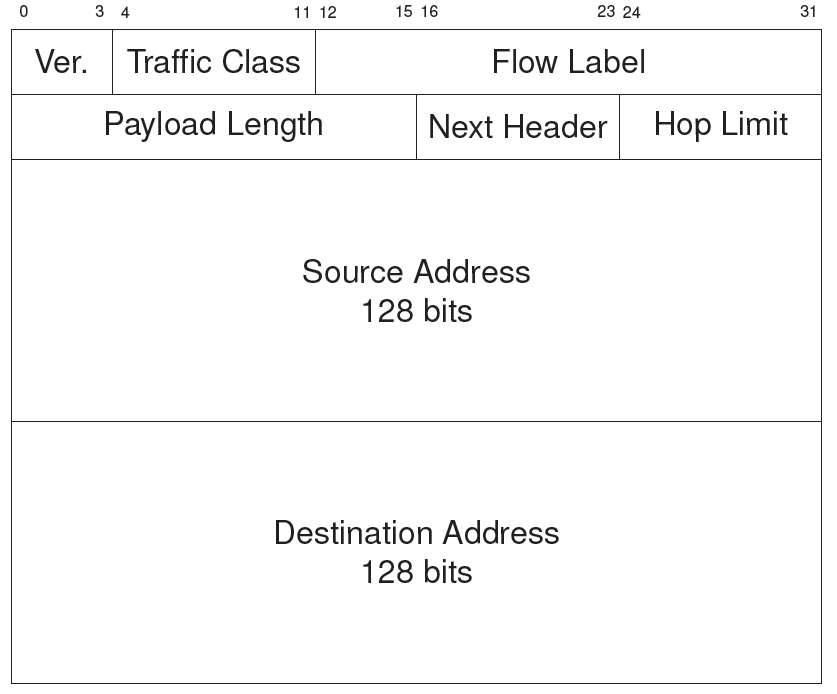
\includegraphics[scale=0.5]{img/ipv6_header.png}
    \decoRule
    \caption{IPv6 simplified packet header structure.}
    \label{fig:ipv6_header}
\end{figure}

It is possible to learn and infer a lot of things from a packet header. Protocols allow the communication between layers; their implementation lies in the header: it is the header that is carrying information, so if we remember it we implicitly know what a protocol does and if it can or cannot do something.

As shown in figure \ref{fig:ipv6_header}, the IPv6 header, with its 320 bits\footnote{IPv4 headers are \textit{at least} 160 bits long: to find the port in such a packet we must check the length of the header and then search for the layer 4 header; there is math to do, which slows down things.}, contains the following information:

\begin{itemize}
    \item \textbf{Version} (4 bits): constant with value equal to 6 (bit sequence 0110);
    \item \textbf{Traffic class} (6+2 bits): the bits of this field hold two values which have the same function as the corresponding IPv4 field. The first six bits hold the differentiated services field (DS field), which is used to classify packets, while the remaining two bits are used for Explicit Congestion Notification (ECN). In other words, this field specifies a packet's priority, so whether it should be enqueued or not, if it should follow a high quality route, and so on;
    \item \textbf{Flow label} (20 bits): a \textit{flow} is group of packets, e.g., a TCP session or a media stream\footnote{IPv4 does not have this field, and in order to check if two packets using this protocol are related we need to check the TCP or UDP ports, meaning that in cases where multiple data streams are related but do not have the same port (such as a video and audio stream sent separately but which should be played together) we have to instruct the router with complex information about how these packets should be used.}; the special flow label 0 means the packet does not belong to any flow. Note that while TCP ports consist of sequences of 32 bits (16 + 16 bits), this field only has 20 bits: this is because this number has been deemed enough in order to correctly label packets. This field is very efficient, and allows the identification of packets to be as simple as a simple XOR operation;
    \item \textbf{Payload length} (16 bits): size of the payload, including any extension headers;
    \item \textbf{Next header} (8 bits): Specifies the type of the next header, usually the transport layer protocol used by a packet's payload. When extension headers are present in the packet, this field indicates which extension header follows. The values are shared with those used for the IPv4 protocol field, as both fields have the same function;
    \item \textbf{Hop limit} (8 bits): replaces the IPv4 \textit{time to live} field\footnote{IPv4's time to live is measured in seconds (or microseconds).}. This value is decremented by one at each forwarding node, and the packet is discarded if it becomes 0. However, the destination node should process the packet normally even if received with a hop limit of 0;
    \item \textbf{Source address} (128 bits): IPv6 address of the sending node;
    \item \textbf{Destination address} (128 bits): IPv6 address of the destination node(s).
\end{itemize}

The most notable things about the IPv6 header are:

\begin{itemize}
    \item \textbf{fixed length} (40 bytes, or 320 bits);
    \item no more error checking (IPv4 had a checksum just for the header, which had to be checked at each node, slowing routing down);
    \item no more fragmentation (at least not in the header itself);
    \item \textbf{header extensions}: it is not wrong saying that IPv6, too, could have layer 4 information (ports) in the header, making things more complex to translate; the difference with IPv4, however, lies in the fact that we know exactly \textit{where} to find this information, making it an extremely simple operation. The process goes like this: after reading the first 40 bytes of a packet, the router checks if the next header has all zeros; if it finds something different from a zero (a 1), then there is one (or more) hop-by-hop extension(s) which has to be further processed, as shown in figure \ref{fig:ipv6_header_pointers};
    \item better support for QoS tags, thanks to the flow control label;
    \item native IPSec\footnote{\textbf{Internet Protocol Security} (IPsec) is a network protocol suite that authenticates and encrypts packets of data to provide secure encrypted communication between two computers over an Internet Protocol (IP) network. It is used in virtual private networks (VPNs).}: the IPv6 specifications say that every host using IPv6 has to also implement IPSec, but it actually is a really complex protocol with a complex key management (to put it simply, a nightmare), so very few systems actually use it;
    \item mobile IPv6\footnote{\textbf{Mobile IP} is the capability of a device using the IP protocol to switch from one network to another (e.g. from 4G to 3G, from a WiFi network to another, etc.) without losing connection because the IP address changes. In a ISO/OSI world this would not happen, because addresses pertaining to different layers would be logically separated (thanks to information hiding), and the session layer would manage exactly this kind of issues. IP has this issue because it exposes the layer 3 address.} greatly simplified, as it keeps the old IP address even on a new network, meaning that the connection will not drop.
\end{itemize}

\begin{figure}[h]
    \centering
    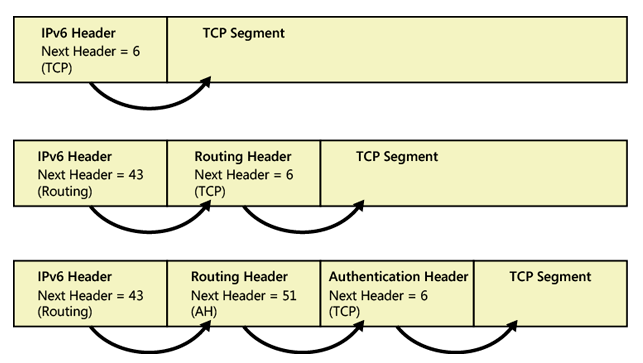
\includegraphics[scale=0.8]{img/ipv6_header_pointers.png}
    \decoRule
    \caption{
    The chain of pointers formed by the Next Header field for various IPv6 packets. In a typical IPv6 packet, no extension headers are present. If special handling is required by either intermediate routers or the destination, the sending host adds one or more extension headers. The Next Header field in the IPv6 header and zero or more extension headers form a chain of pointers. Each pointer indicates the type of header that comes after the immediate header until the upper-layer protocol is ultimately identified.}
    \label{fig:ipv6_header_pointers}
\end{figure}

%-------------------------------------------

\subsection{Autoconfiguration}
This is the strongest point of IPv6, which must never be underestimated for security purposes, because the more a system is user-friendly, the more it is actually dangerous.

The idea of IPv6's autoconfiguration is to just plug the cable in and have everything automatically working (\textbf{plug \& play}), without the user's intervention. This behavior is based first and foremost on auto negotiation of IP addresses which, unlike IPv4, is done without the help of DHCP\footnote{\textbf{DHCP}, or Dynamic Host Configuration Protocol, is a network protocol used on IP networks where a DHCP server automatically assigns an IP address and other information (namely, the subnet mask, default gateway address, domain name server (DNS) address and other pertinent configuration parameters) to each host on the network so that they can communicate efficiently with other endpoints. DHCP is an essential method to ensure that devices are able to join networks and are configured correctly, and greatly reduces the errors that are made when IP addresses are assigned manually. It can also stretch IP addresses by limiting how long a device can keep an individual IP address.} (although it can still be used in IPv6, too).

%----------------------------------------------------------------------------------------

\section{IPv6 addressing}
The IPv6 address space is so large that a new addressing scheme is needed. The two RFCs that define it are:

\begin{itemize}
    \item \textbf{RFC 4291}: defines the IPv6 addressing scheme;
    \item \textbf{RFC 3587}: defines the IPv6 global unicast address format.
\end{itemize}

IPv6 addresses are written using the \textbf{hexadecimal} format (base 16). An IPv6 network card always has several IPv6 addresses.

There are many types of IPv6 addresses:

\begin{itemize}
    \item \textbf{unicast}: one-to-one address, which can be of one of the following types:
    
    \begin{itemize}
        \item \textbf{global}: its scope is the whole Internet, and it is unique;
        \item \textbf{link-local}: it lives in the link scope, meaning that if two devices are on the same link (e.g. attached to the same switch) they will have this kind of address, which might not be unique. Also, since we have to define the link, there might be a link-local address for every network interface connected to a given device. In a multi-hop network like a wireless network, the scope of the link is the radio range of the network, so the link-local address will be valid only between one device and another that can be reached within one hop. In general, if the devices we are considering work at layer 2 (e.g. have multiple switches), then all hosts will be in the same link\footnote{A regular WiFi access point (with DHCP that gives out IP addresses) will have its devices on one link, while the ones in the wired network on a different one. However, if the access point is configured as a bridge, then everything will be on the same link.};
        \item \textbf{site-local}: deprecated, used before ULA;
        \item \textbf{unique local (ULA)}: extremely limited and specific use, as it is similar to private addresses (e.g. it is used as a temporary solution in cases where we are configuring an IPv6 address but still do not have a valid prefix);
        \item \textbf{IPv4-compatible}: deprecated;
        \item \textbf{IPv4-mapped}: an IPv6 address which has been mapped to IPv4; it is meant as a solution for the IPv6 transition, although it is not a very elegant one.
    \end{itemize}
    
    \item \textbf{multicast}: one-to-many, an address that allows a device to talk to many other devices at the same time; it is used for almost everything\footnote{In IPv4 it is not commonly used, as it is complex for routers to split the data when receivers are on different networks (and in general, it is not a simple operation), and the multicast's usefulness is extremely limited.};
    \item \textbf{anycast}: one-to-nearest; it works much like a unicast address, except that data is sent to the nearest host (so destination is decided by the router). There can be more than one device that are globally reachable at the same distance. Anycast is widely used for content delivery network products (CDN, a geographically distributed network of proxy servers and their data centers) in order to bring their content closer to the end user, because it is far more efficient than checking a list of IPv4 addresses to find out which is the nearest.
\end{itemize}

There is no broadcast address, because multicast is a lot more powerful.

%-------------------------------------------

\subsection{IPv6 address format}

The preferred format for a 16-byte global IPv6 address is as shown in the following example (extended and compact form):
\begin{center}
    \texttt{2001:0DB8:3003:0001:0000:0000:6543:210F}
    
    \texttt{2001:DB8:3003:1::6543:210F}
\end{center}

The \textbf{compact form} shown below the full one omits all leading zeros, keeping just the colons in order to avoid ambiguity in the address' length.

There also exists a \textbf{literal representation} which uses square brackets and can be used to insert the address in, for example, an HTTP address (just like we can do with an IPv4 address):
\begin{center}
    \texttt{[2001:DB8:3003:2:a00:20ff:FE18:964c]}
    
    \emph{} \texttt{http://[2001:DB8:3003:2:a00:20ff:FE18:964c]:80/index.html}
\end{center}

\emph{Example} A curious use of IPv6 prefixes, and a good example of why we can say that the IPv6 address space is so large that we can afford to actually waste addresses, is the \textbf{Debate Prefix}, or \textbf{2001:DB8::/32}. This is an address prefix that is only used for \textit{documentation}, so addresses beginning with this prefix cannot be routed (routers automatically drop packets containing them as destinations). Note that there are $2^{96}$ addresses reserved just for this purpose: a significant waste of addresses. In spite of this, this prefix is necessary in order to avoid wrongly configured networks (even at ISP levels) created by people who copy-pasted examples without changing IP addresses.

%-------------------------------------------

\subsection{IPv6 address prefixes}
The currently IANA\footnote{The \textbf{Internet Assigned Numbers Authority} (IANA) is a standards organization that oversees global IP address allocation and other Internet Protocol-related symbols and Internet numbers.} allocated prefixes are:

\begin{itemize}
    \item \textbf{\texttt{::/128}} (all zeroes): unspecified (special cases only);
    \item \textbf{\texttt{::1/128}}: loopback (there is no place like \sout{home} \texttt{::1/128});
    \item \textbf{\texttt{2000::/3}}: global unicast addresses (RFC 4291); anycast addresses are allocated from unicast prefixes, so they are indistinguishable;
    \item \textbf{\texttt{FC00::/7}}: unique local unicast, almost never used (link-local addressed are used in their place) (RFC 4193);
    \item \textbf{\texttt{FE80::/10}}: link-local unicast (RFC 4291);
    \item \textbf{\texttt{FF00::/8}}: multicast (RFC 4291);
    \item \textbf{\texttt{64:FF9B::/96}}: IPv6-mapped IPv4 address (RFC 6052);
\end{itemize}

%-------------------------------------------

\subsection{Link-local addresses}
In order to get a global unicast address we need to know some data about the network that we are joining.

The link-local unicast address, vice versa, does not require us to know anything in particular, because it is used on the local link: this kind of address is used during autoconfiguration, even when no routers are present.

\begin{figure}[h]
    \centering
    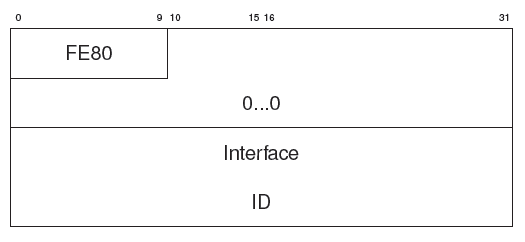
\includegraphics[scale=1]{img/ll.png}
    \decoRule
    \caption{Link-local address structure.}
    \label{fig:ll}
\end{figure}

As shown in figure \ref{fig:ll}, the first 10 bits of a link-local address are always \texttt{FE80}, while the next 54 bits are filled with zeros (could also be ones though, it would still be valid). The second part, made of the remaining 64 bits, is filled with the \textbf{interface ID}, which must be unique (every device must have a different interface ID).

%----------------------

\subsubsection{Interface ID}
The simplest way to obtain a unique interface ID is to use the MAC address of the device, since on the same link it also has to be unique for every NIC, and thus we can use this to build a layer 3 address.

However, the interface ID can also be built in other ways. For example, if we have a shorter MAC address (like in Ethernet or WiFi networks) we will have to expand it to 64 bits, thus creating an EUI-64 address.

We could also generate addresses using DHCPv6 (slightly more complex than DHCPv4 because of how hosts are identified), configure them manually or generate them with pseudo-random numbers (in this case the probability that two hosts select the same numbers is extremely low).

We can also generate it in a more creative way, like in the case of CGAs (Cryptographically Generated Address), which are generated using the 64 bits of the cryptographical signature of our data packets.

Other methods include basically anything that can be used to generate a reasonably unique address; we should make sure, however, to always double-check everything, just in case.

\begin{figure}[h]
    \centering
    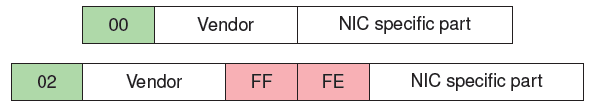
\includegraphics[scale=1]{img/autonconfexample.png}
    \decoRule
    \caption{Example of autoconfigured IPv6 address (bottom) using a 48-bit MAC address (top). The MAC address 00:1F:5B:39:67:3C maps into the IPv6 address \texttt{{\color{red} 02}1F:5B{\color{red}FF:FE}39:673C.}}
    \label{fig:autonconfexample}
\end{figure}

%-------------------------------------------

\subsection{IPv6 interfaces}
Each host (computer) with at least one NIC has \textit{at least three} IPv6 addresses:

\begin{itemize}
	\item \textbf{loopback} (\texttt{::1/128}): the IPv6 equivalent of the \textit{localhost} address in IPv4, assigned to a virtual network interface card called loopback;
	\item \textbf{link-local unicast address} (\texttt{FE80:::::}): each MAC address configured for each NIC has its own link-local address;
	\item \textbf{global unicast}\textit{s}: assigned in some way, there could be more than one per device;
	\item \textbf{all-nodes multicast} (\texttt{FF02::1}): the device might also reply to one or more multicast addresses, which are the equivalent of an IPv4 broadcast address;
	\item \textbf{all-routers multicast} (\texttt{FF02::2}): routers also have all-routers multicast address;
	\item \textbf{solicited-node multicast address} (\texttt{FF02::1:FF00:0000/104}): the core and culprit of autoconfiguration. Such an address is an IPv6 multicast address valid within the local-link, and is used in the Neighbor Discovery Protocol for obtaining the layer 2 link-layer addresses of other nodes. A solicited-node multicast address is created by taking the last 24 bits of a unicast or anycast address and appending them to the prefix \texttt{FF02::1:FF00:0/104}. We use a solicited multicast group instead of the all-node address because the all-nodes group could be too numerous, and constantly being talked to by somebody joining the network would greatly reduce efficiency; by using solicited-node multicast addresses we are limiting the target to a very small subset of the nodes.
\end{itemize}

Note that when using different addresses to specify high-level capabilities of a node, we are actually transferring layer 7 (application) functions to layers 2 and 3: a further betrayal of the principle of separation of concerns.

\vspace{0.5em}

\emph{Example} If we want to reach a printer we use an \textit{all-printer multicast address} - which is actually great, because we do not have to ask every single node if they have one of the (zillion) protocols supported by printers; instead, we send just a packet and reach all of them at the same time.

The same goes for finding a DHCP server: we send a packet to an \textit{all-DHCP multicast address} and it will reach only nodes which implement DHCP.

\vspace{0.5em}

%----------------------

\subsubsection{IPv6 multicast groups}
What does joining a multicast group actually mean?

Let us suppose that we are joining a \texttt{FF02} group: we just have to instruct our IP layer that the packets that have such an address as destination must not be discarded, but passed through the IP layer itself towards the upper layers (it is a sort of filtering). This is actually the reason why multicast addresses are more efficient than broadcasts: packets will be discarded earlier in the stack by nodes that are not routers; any node can send packets to a multicast group, but those who are not part of the group will discard packets at IP layer (in the kernel, in an earlier and faster way). In other words, IPv6 uses the broadcast address at layer 2, so if we join a link-local scope, we only have to grab the IPv6 address that we are sending stuff to, tell to layer 2 to transform it into a MAC address, and then send it. By contrast, in IPv4 the broadcast address (an IP/layer 3 address) is mapped to a layer 2 address, meaning that every node will receive it; a switch will send a broadcast packet to all ports, and all NICs will forward it to the IP layer.

It is clear thus that the node does not need anything to join a multicast group. Depending on the \texttt{02} bit, it might not even need to tell anybody: the IPv6 multicast address has a scope (reachability) defined by that bit, meaning that while \texttt{01} is \textit{interface local} (the packet will not even go outside the NIC), \texttt{02} has link-local scope. 

Other multicast scopes are \textit{realm-}, \textit{admin-}, \textit{site-}, \textit{organization-} local; these are not on a link, so packets will pass through routers and when joining one of these groups we will have to tell the router that we are part of that group.

In general, there is \sout{a shitload} quite a large number of multicast address types, and we could define even more of them.

%-------------------------------------------

\subsection{Autoconfiguration (again)}
Autoconfiguration is very simple, and very vulnerable. We have seen how to read IPv6 addresses, and that there are multiple classes of IPv6 addresses (the most important ones are global, link-local and multicast addresses). In order to better understand it, we are going to see how it works in practice.

For any node, autoconfiguration can be summarized in the following steps:

\begin{enumerate}
    \item build the \textbf{interface ID} (node ID, with any of the methods seen earlier);
    
    \item join the \textbf{solicited-node multicast address group}, and send out a \textbf{DAD} (Duplicate Address Detection) message; the DAD is not sent with the node's source address, because it still does not know if it can use it or not, so instead it uses an unspecified (all zeros) address as source. The node then waits for a response until a timeout expires; anyone who is already using that address must reply to the DAD request, while if the node does not receive anything back then it will assume that the chosen address is safe to use (implicit acknowledgement);
    
    \item start using the link-local address to check for Router Advertisements (RA), ICMP\footnote{Internet Control Message Protocol, a protocol used by network devices to send error messages and operational information indicating success or failure when communicating with another IP address.} messages periodically sent to the all-node multicast group by routers (with a \textit{still alive} kind of function);
    
    \item build a global unicast address: if there is no DHCP, RAs contain a PIO (Prefix Information Object) telling the node which prefix it can use in order to build a global address; otherwise, RAs contain a flag indicating that the node should rely on the DHCP in order to get a global address (which leads to using an all-DHCP multicast group). RAs also contain the DNS;
    
    \item send another DAD (only if there is no DHCP, otherwise the node trusts that the DHCP gave it a unique address);
    
    \item automatically set a default router\footnote{In IPv4 this was either set by the DHCP, or it had to be manually configured.};
    
    \item start surfing the Internet.
\end{enumerate}

The second step of the process represents a problem on multiple levels, because there might be a node who does use the chosen address, but replies too late. The optimal value for the timeout should then be a compromise between speed and safety, so it depends heavily on the network topology; usually, for Ethernet and WiFi it does not matter much, because replies will be in the order of milliseconds, but for long-distance/long-delay systems it is very important.

During this step the node also implicitly assumes that the DAD (which is an UDP-like packet) will be received by every node, and thus that the network is reliable; in a network with a high probability of packet loss, this system is unreliable.

Last but not least, the node \textit{also} assumes that there are no attackers that might reply in a funky way. However, if there actually \textit{is} an attacker in the network, he/she could easily prevent a node from joining the network by simply joining all solicited-node multicast groups him/herself and constantly replying to anyone else trying to join that the IPv6 address they would like to use has already been claimed. Assuming that there are no sons of bitches around, then the node will start using its own link-local address.

\vspace{0.5em}

\emph{Example} Suppose we have an interface with the IP address \texttt{FE80::2AA:FF:FE28:9C5A}. Since a solicited-node multicast address is created by taking the last 24 bits of a unicast or anycast address and appending them to the prefix \texttt{FF02::1:FF00:0/104}, the associated solicited-node multicast address is \texttt{FF02::1:FF28:9C5A}. Note how, having taken 104 bits from the address, the last byte of the penultimate field \texttt{00} is not used in the prefix.

It is interesting noting that the solicited-node multicast address prefix \texttt{FF02} is also used in the autoconfiguration for the global multicast addresses; a subset of 24 bits of the original address, however, is large enough to have an extremely small probability to get a DAD reply, even from someone with a very similar address.

\vspace{0.5em}

The DNS is usually got from the RA, but can also be:

\begin{itemize}
    \item obtained from the IPv4 stack, if there is a dual-stack;
    \item manually configured (definitely a bad idea);
    \item obtained from DHCPv6;
\end{itemize}

Note that in old machines or custom made IP stacks we have to double check that they understand RAs or DHCP with DNS, otherwise our devices will apparently work, but they will not be able to resolve addresses.

%----------------------

\subsubsection{About autoconfiguration attacks}

What happens if an attacker gets into this process? Total panic: there is no way to avoid it. The most dangerous attacks are those on the same link, where one usually assumes that no attacker can get that close to a victim. Some people proposed to secure on-link messages with a cryptographic protocol, but this would go against autoconfiguration, because it would require that every device that can join the network has already been configured for that network (given a secret). So in short, we either have autoconfiguration, or we protect ourselves from attackers: it is a short blanket.

%----------------------

\subsubsection{More about IPv6 vs. IPv4}
In general, we must forget about many concepts bound to IPv4, because they are utterly wrong in IPv6. As an example, in IPv6 there is no netmask, because the address is simply split between a net part (which is always 64 bits long) and the network interface part (made of the other 64 bits), so we cannot ever have subnets of different length and sizes.

Neighbor solicitation is another example: while in IPv4 it is enabled when two hosts share the network part, this is not always true in IPv6, because when a node has a unicast packet to send to a neighbor but does not know the neighbor’s link-layer address, it performs address resolution.

Note that in IPv6 neighbors are nodes attached to the same \textbf{link}, which is defined as \textit{a communication facility or medium over which nodes can communicate at data link layer, i.e. the layer immediately below IP}. This means that everything depends on the layer 2 physical topology, not on something that we can infer from the IP address.

The only concept that holds is \textit{on-link}, which is not based on the IP address. But still, while in IPv4 two addresses are in the same subnet if they share the same network part (and thus they are connected by a switch or another layer 2 system, and do not need a router), in IPv6 we can never infer from two IP addresses if they are attached to the same switch, if there is a router in between and/or if they can communicate directly, even if they ping each other. The on-link property is \textit{not} a consequence of having the same prefix.

\vspace{0.5em}

\begin{figure}[h]
    \centering
    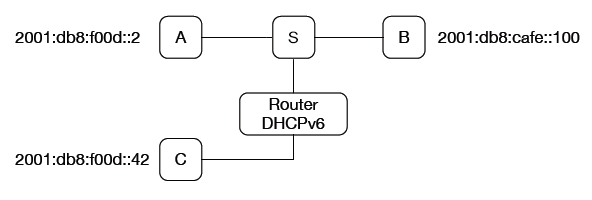
\includegraphics[scale=0.7]{img/neighbors_example.png}
    \decoRule
    \caption{IPv6 on-link example.}
    \label{fig:neighbors_example}
\end{figure}

\emph{Example} Let us consider the network shown in fig. \ref{fig:neighbors_example}: devices A and B are on the same link but have different IP address prefixes, while A and C are on different links but have the same prefixes.

In IPv4, devices A and B would not be able to communicate, because their addresses do not have the same prefix. Additionally, having A and C with the same prefix or the same network part on two different sides (physical interfaces) of the router would create a dramatic conflict: the router would be quite unhappy; it is possible, but only if he have very good hands and we build the routing table in a very specific way, not only on the router, but also in A and C - basically, it would be a bad idea.

In IPv6, vice versa, not only the network in the figure is legal, but also all devices will communicate with each other: A and B because they are on the same link (connected by switch S), while A and C because they know that they are attached to the same router.

It is the router who tells in its Router Advertisement (RA) to the A-B link that they are on the same link (connected by the router itself), by means of a prefix and an on-link bit which, if set, allows every host to assume that any other host that share the same prefix is on the same link (IPv4-alike). If the on-link bit is not set, then no host will ever assume that a given destination is on the same link, unless the router will them otherwise.

Let us suppose now that A wants to send a packet to C; since A does not assume that C is on the same link, it will send it to the router, which will forward it to C. C will do the same.

If A and B would do this operation, too, then it would be sub optimal: every packet will pass through the router, while it could simply go from A to B (and vice versa) directly, since they are on the same link.

Suppose now that there is another host D, with the IPv6 address \texttt{2001:db8:f00d::66}\footnote{Read \textit{"two-thousand debate food"}.}, on the same side as C; in this case A will send its packets to the router, which will forward them to D, and D will do the same with packets destined to A. This, too, is sub optimal, since data will have to go through the router.

\vspace{0.5em}

%-------------------------------------------

\subsection{ICMP redirect}
We said earlier that autoconfiguration is a very sensible spot of IPv6. The truth is that there is another phenomenal vulnerability in this protocol, and this is ICMP (Internet Control Message Protocol) redirect.

Through ICMP, the router can inform a device about the on-link property of a destination, effectively redirecting packets.

\vspace{0.5em}

\emph{Example} Let us consider the example in figure \ref{fig:neighbors_example} again.

Suppose that A sends a packet to B through the router. The router forwards the packet to B \textit{and} sends a message (to B) telling it that A is on-link, and giving it A's MAC address. From there on, A and B will know that they are on the same link and thus A will send packets directly to B, and vice versa.

Now, suppose that B is a router with a slightly different address (another number instead of the final \texttt{100}). If A does not know that B is the right router, it will send a packet to the main router; the main router will forward the packet \textit{and} send a message to A telling it that the designated router is B, so that from there on A will send packets directly to B.

\vspace{0.5em}

The example above explains how ICMP redirect works; the vulnerability lies in the fact that if we have an attacker on a given link that forges fake redirect messages, he/she can claim to be the router for a given block of addresses and for any host on the Internet, thus bypassing all routers after the first package (because hosts will work at switch level).

The point is that we can have completely different addresses that communicate directly if a router (or someone who poses as a router) tells them that they are on the same link.

In short, ICMP redirect is an extremely powerful mechanism, but very dangerous, too. In spite of this, it is dramatically useful and important in order to set up and maintain a network with multiple routers and addresses, because even if we could skip (filter) its messages, it would be a very bad idea.

%----------------------

\subsubsection{Countermeasures}
Given the \textit{huge} vulnerability represented by ICMP redirect, we need to have a security plan. Remember that \textit{security} is not about making things secure, but rather about defining what security means for us - and making it happen.

The steps to reach the target security must follow a precise path:
\begin{itemize}
    \item understand the enterprise architecture and its goals;
    \item define the security targets that have to be enforced (e.g. robustness, failsafe operation and percentage, admitted outage, confidentiality, etc.);
    \item analyze threats, occurrence probability and attacker capabilities;
    \item define countermeasures;
    \item measure the effectiveness.
\end{itemize}

In the case of IPv6, we have to evaluate if the link-local network can be physically touched by somebody that is not trusted (for example, the university's network is not trustable because some ports are located in rooms that are publicly accessible, like the Ethernet port in the printing room).

A countermeasure to ICMP redirect attacks could be controlling what passes through the network - physically-wise. We should check that the network cable is physically secure (e.g. in an iron tube), in order to make sure that it is always sane and cannot be touched; periodical electrical checks (a fairly common solution) could also be employed to ensure that it has not been detached and reattached.

We could also check where a packet comes from: against somebody who pretends to be a router we could install a check on the switch to see on which port is located the router, and only allow RA messages from that port (meaning that everything else is an attacker). However, in order to do this we need to have a switch able to analyze this kind of threat.

%-------------------------------------------

\subsection{IPv6 threat model}
IPv6 attacks can be divided in two main categories:
\begin{itemize}
	\item IP-level attacks and vulnerabilities;
	\item upper-layer attacks and vulnerabilities.
\end{itemize}

Upper-layer attacks and vulnerabilities are not our business, but we should always check for possible holes in the software. IPv6 addresses (and in particular IPv4-mapped ones), on the other hand, can (and \textit{will}) raise application-level vulnerabilities.

Compared to IPv4, IPv6 has some similar attacks, but also some new ones. There are many IPv4 attacks that do not apply to IPv6 anymore.

For example the fragmentation attack, which is possible in IPv4, is impossible in IPv6 - not because IPv6 does not have fragmentation, but because on IPv6 the extension header for destination is end-to-end (only the source can fragment packets): if we find a malformed packet, we can easily assume that either the sender went nuts or the sender is kinda sus, so we just trash it (fig. \ref{fig:fry_packet}).

Network scanning is also practically impossible in IPv6 if the attacker is not in the same network because of the huge dimensions of the address space - this also means that the network is harder to control, though.

Another nice thing is that NATs are gone; however, since networks still need to be partitioned, IPv6 uses more firewalls than IPv4.

\begin{figure}[h]
    \centering
    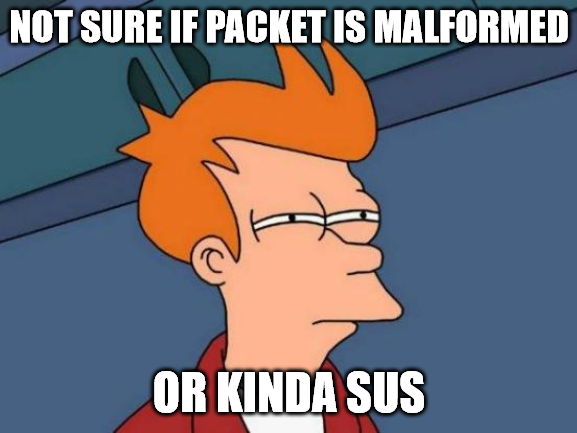
\includegraphics[scale=0.6]{img/fry_packet.png}
    \decoRule
    \caption{A router trying to figure out if a given packet is malformed or has been tampered with.}
    \label{fig:fry_packet}
\end{figure}

The ICMP redirect attack is, vice versa, a new kind of attack that was not possible in IPv4, while ARP spoofing\footnote{Address Resolution Protocol spoofing, an IPv4 attack where an attacker is able to make a certain destination believe that he/she is somebody else.} is still there, even though in a slightly different form.

The point is that IPv6 has not been created to be secure, but only to be easier to use than IPv4; being made to be easier for the user means that it is easier to exploit for the attacker. The fact that something has been certified as secure (with a given level of security) on IPv4 does not imply a similar level of security in IPv6. Obviously, assuming that systems are similarly secure in both IPv4 and IPv6 would be a horrible mistake. For this reason, because IPv4 and IPv6 are completely unrelated, in order to check if a software/protocol is secure at layer 3 or - even more importantly - layer 7, we need to make a \textbf{vulnerability assessment}, or \textbf{vulnerability analysis} (check for memory leaks and other problems that arise from the fact that IPv6 addresses are longer) for both of them.

Remember: IPv6 is \textbf{not} more secure than IPv4; it is just \textit{differently insecure} (also, we do not even have much experience with IPv6 attacks, so it is harder to make it more secure).

\vspace{0.5em}

\emph{Example} The THC IPv6 Attack Toolkit comes with lots of effective IPv6 attacking tools; it can be found at \url{https://github.com/vanhauser-thc/thc-ipv6}.

\vspace{0.5em}